\chapter{Cross Section Measurement}\label{chapt:xsec}

The cross section measurement procedure and results are explained in this section.
After applying selection criteria and kinematic reconstruction, one can count the events to determine
the rate of the $t\bar{t}$ production process.

The cross sections were measured double differentially in bins of the kinematic variables of the top-quark and the $t\bar{t}$ system.
The first section shortly describes the way how the background yields were subtracted.
The two dimensional unfolding applied to correct for the detector effect and fluctuations is described
in the second section.
The double differential cross sections and their definitions are shown in the last section of the chapter.
% \section{Selection of Binning}\label{sec:binning}

\section{Background Subtraction}
This study is performed as counting the events which fulfill certain criteria (e.g. given in chapter \ref{chapt:event_selection} and 
chapter \ref{chapt:kinReco}). 

\begin{equation}\label{eq:bgsub}
 N^{signal\;measured}_{reco} = N^{selected}_{reco} - N^{BG}
\end{equation}

Here $N^{BG}$ corresponds to the estimated number of background events. The background sources were introduced in sec. \ref{sec:bg_intro}.

After subtracting all the non-$t\bar{t}$ backgrounds, the number of signal events is multiplied by a factor to correct for the contribution
from other decay channels of $t\bar{t}$:

\begin{equation}\label{eq:bgsub}
 N^{signal}_{reco} = N^{signal\;measured}_{reco} \cdot \frac{N^{t\bar{t} \rightarrow e\mu}_{reco}}{N^{t\bar{t} \rightarrow e\mu}_{reco} + N^{t\bar{t} \rightarrow other}_{reco}}.
\end{equation}

The whole factor $\frac{N^{t\bar{t} \rightarrow e\mu}_{reco}}{N^{t\bar{t} \rightarrow e\mu}_{reco} + N^{t\bar{t} \rightarrow other}_{reco}}$ was derived
from the simulated data.

%%%%%%%%%%%%%%%%%%%%%%%%%%%%%%%%%%%%%%%%%%%%
%%%%%%%%%%%%%%%%%%%%%%%%%%%%%%%%%%%%%%%%%%%%
%%%%%%%%%%%%%%%%%%%%%%%%%%%%%%%%%%%%%%%%%%%%
\section{Unfolding of the Experimental Results}\label{sec:unfold}

The signal yields after the background  subtraction \ref{eq:bgsub} are grouped to the bins in different variables. However, the kinematic properties
of the events are measured with finite precision due to inevitable detector effects and imperfect reconstruction algorithms.
Thus, some fraction of events may be reconstructed in the wrong bins. To present the results independent of the detector effects,
one needs to correct them back.

The whole problem can be described as

\begin{equation}\label{eq:UnfoldProb}
 \tilde{y}_i = \sum_{j = 1}^{m} A_{ij}\tilde{x}_{j} + b_{i}, \;\;\; 1 \leq i \leq n.
\end{equation}

Here the $\tilde{x}_j$ in $m$ bins denotes the true distribution, independent of the detector effects, which is the aim of the measurement;
$\tilde{y}_i$ in $n$ bins is the distribution which one gets out of the detector and $A_{ij}$ is a matrix of probabilities describing 
the migrations from true leven bin $j$ to detector level bin $i$ to different bins on the detector level; $b_{i}$ is the background in the bin $i$. 
However, the observed event counts $y_{i}$ may be different from $\tilde{y}_{i}$ due to the statistical fluctuations.
A schematic view of the problem is given in the Figure \ref{fig:scUnf}.

\begin{figure}[t]
  \centering
  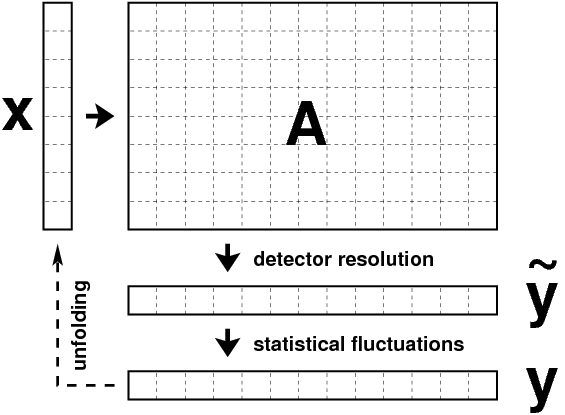
\includegraphics[width=0.4\textwidth]{06_DiffXsec/plots/d12-129f1.png}
  \caption{Schematic view of the problem of migration effects due to the finite precision of the detector and statistical 
  fluctuations. Plot taken from \cite{Schmitt:2012kp}.}
  \label{fig:scUnf}
\end{figure}

The process of estimating the true distribution $\tilde{x}_{j}$ from the observed distribution $y_{i}$ which was influenced
by detector effects is called \textit{unfolding}. To minify the statistical fluctuations the smoothing  
\textit{regularisation} procedure is applied. The TUnfold \cite{Schmitt:2012kp} algorithm was used for the
unfolding in this analysis.

\subsection{TUnfold Minimization}\label{ssec:TUmini}

The TUnfold algorithm is using a method based on least square minimization plus Tikhonov regularization \cite{Tikhonov:1963}. One of the ingredients 
for a good performance of the method is that the number of degrees of freedom for the minimization ($n - m$) has to be positive,
or $n > m$. This means that the unfolded distribution $\tilde{x}_j$ will have coarser binning than the measured one, $y_{i}$.

The unfolding algorithm of the TUnfold determines the stationary point or minimum of the following Lagrangian:

\begin{align}
 \mathcal{L}(x, \lambda) & = \mathcal{L}_{1} + \mathcal{L}_{2} + \mathcal{L}_{3}, \;\;\;\;\;\;\;\;\;\; \textrm{where}\\
 \mathcal{L}_{1} & = (\mathbf{y} - \mathbf{A}\mathbf{x})^{T} \mathbf{V_{yy}}^{-1}(\mathbf{y} - \mathbf{A}\mathbf{x}),\\
 \mathcal{L}_{2} & = \tau^{2}(\mathbf{x} - f_{b}\mathbf{x_{0}})^{T} (\mathbf{L^{T}L}) (\mathbf{x} - f_{b}\mathbf{x_{0}}), \\
 \mathcal{L}_{3} & = \lambda(Y -\mathbf{e}^{T}\mathbf{x}) \;\;\;\;\;\;\;\;\;\;\;\;\;\;\;\; \textrm{with} \\
 Y & = \sum_{i} y_{i}, \\
 e_{j} & = \sum_{i} A_{ij}.
\end{align}

The bold symbols here correspond to matrices and vectors.

The term $\mathcal{L}_{1}$ is expected for a least square minimization. The vectors $\mathbf{y}$, $\mathbf{x}$ and the matrix $\mathbf{A}$ were
described in the previous section. Representing the migrations into different bins of $\mathbf{y}$, the matrix $\mathbf{A}$
is defined from the $t\bar{t}$ signal Monte Carlo simulation\footnote{The matrix $\mathbf{\tilde{A}}$ is
determined from Monte Carlo using the information from the generator particle level and on the reconstructed level. It describes how many 
migrations there are out and into a certain bin. An extra "zero`` row is added
to the matrix $\mathbf{\tilde{A}}$ containing the information about the count of Monte Carlo events which were generated in some bin of $\mathbf{x}$,
but were not reconstructed in any of the $\mathbf{y}$ bins. \\ The matrix $\mathbf{A}$, which enters the unfolding, is the normalized $\mathbf{\tilde{A}}$
defined as $\mathbf{A}_{ij} = \frac{\tilde{A}_{ij}}{\sum_{j=0}\tilde{A}_{ij}}$ (the normalization includes the "zero'' row).}. An example of such matrix 
is shown in fig. \ref{fig:migMat}. 

\begin{figure}[p]
  \centering
  \includegraphics[width=1.0\textwidth]{/home/dolinska/Dropbox/desy_plots/Thesis/Jenya/xSec/migration/probMatrix_top_arapidity_top_pt.pdf}
  \caption{Normalized migration matrix $\mathbf{A}$ (probability matrix) in bins of $p_{T}(t)$ and $|y(t)|$. The generated binning is the following:
          the sequences of three bins (1-3, 4-6, 7-9, 10-12, 13-15) correspond to the $p_{T}(t)$ bins $[0\:\:65\:\:130\:\:200\:\:300\:\:500]$ GeV.
          There are 3 $M(t\bar{t})$ bins -- $[340\:\:450\:\:600\:\:1000]$ GeV -- in each $p_{T}(t)$ bin.
          Detector binning:
          the sequences of eight bins (1-8, 9-16, 17-24, 25-32, 33-40, 41-48, 49-56, 57-64, 65-72, 73-80, 81-88, 89-96, 97-104, 105-112) correspond 
          to the $p_{T}(t)$ bins $[0\:\:20\:\:35\:\:50\:\:65\:\:80\:\:100\:\:130\:\:145\:\:170\:\:200\:\:240\:\:300\:\:350\:\:500]$ GeV.
          There are eight $|y(t)|$ bins -- $[0.0\:\:0.2\:\:0.4\:\:0.6\:\:0.8\:\:1.0\:\:1.2\:\:1.5\:\:2.5]$ -- in each $p_{T}(t)$ bin.}
  \label{fig:migMat}
\end{figure}

% \begin{figure}[p]
%   \centering
%   \includegraphics[width=1.0\textwidth]{/home/dolinska/Dropbox/desy_plots/Thesis/Jenya/Plots/Nominal/emu/top_arapidity-top_pt/probabilityMatrix_top_arapidity_vs_top_pt.pdf}
%   \caption{Migration matrix for the bins of $p_{T}(t)$ and $|y(t)|$. The binning is the following:
%   X axis: the sequences of three bins (1-3, 4-6, 7-9, 10-12, 13-15) correspond to the $p_{T}(t)$ bins $[0\:\:65\:\:130\:\:200\:\:300\:\:500]$ GeV.
%           There are 3 $|y(t)|$ bins -- $[0\:\:0.6\:\:1.2\:\:2.5]$ -- in each $p_{T}(t)$ bin.
%   Y axis: the sequences of eight bins correspond to the $p_{T}(t)$ bins $[0\:\:20\:\:35\:\:50\:\:65\:\:80\:\:100\:\:130\:\:145\:\:170\:\:200\:\:240\:\:300\:\:350\:\:500]$ GeV.
%           There are 8 $|y(t)|$ bins -- $[0\:\:0.2\:\:0.4\:\:0.6\:\:0.8\:\:1.0\:\:1.2\:\:1.5\:\:2.5]$ -- in each $p_{T}(t)$ bin.
%   The matrix is obtained from the \MG + \PYTHIA 6 signal sample.}
%   \label{fig:migMat}
% \end{figure}

The term $\mathcal{L}_{2}$ is responsible for the regularization. It is reducing the effect of the statistical fluctuations from $\tilde{\mathbf{y}}$ on $\mathbf{x}$
during the search of the stationary point of the Lagrangian $\mathcal{L}$. The $\tau^{2}$ is the regularization strength. The matrix $\mathbf{L}$
represents the so-called regularization conditions, having $n$ columns and $n_{R}$ rows which corresponds to $n_{R}$ conditions. $f_{b}$ is a normalization 
factor and $\mathbf{x_{0}}$ is the bias vector. In a very simple case $f_{b} = 0$, $\mathbf{L}$ is a unity matrix and $\mathcal{L}_{2} = \tau^{2} \parallel x \parallel^{2}$, which
suppresses large deviations of $\mathbf{x}$ from zero. In case $f_{b} = 1$, the deviations of $\mathbf{x}$ from $\mathbf{x_{0}}$ are
suppressed. For this analysis $f_{b} = 1$ is used and $x_{0}$ corresponds to the generated distribution. It is very important to choose 
the optimal regularization strength, as a very weak strength would not damp the fluctuation effects from $\mathbf{y}$, whereas a very strong 
one will bias $\mathbf{x}$ towards $f_{b}\mathbf{x}_{0}$. The L-curve method \cite{Hansen00thel-curve} and the minimization
of correlation coefficients \cite{VBlobelT} are implemented in TUnfold for an optimal regularization strength choice. 

The idea of the L-curve method is to look at the graph $L_{x}^{curve}$ vs $L_{y}^{curve}$ and choose the $\tau$ from the point with
maximal curvature. The $L_{x}^{curve}$ and $L_{y}^{curve}$ are expressed as follows:

\begin{equation}
 L_{x}^{curve} = log \mathcal{L}_{1},
\end{equation}

\begin{equation}
 L_{y}^{curve} = log \frac{\mathcal{L}_{2}}{\tau^{2}}.
\end{equation}

The L-curve graph is in fact comparing the two terms of the Lagrangian: the minimization term $\mathcal{L}_{1}$ and the regularization term $\mathcal{L}_2$.
The maximum curvature point of this L-curve is a point of compromise between the size of the $\mathcal{L}_{1}$ and $\mathcal{L}_{2}$ contributions
to the total Lagrangian.

The method of minimizing the global correlation coefficient chooses the $\tau$ at the point where the average correlation coefficient 
$\sum_{i} \frac{\rho_{i}}{n}$ is minimal. Here $i$ is the component of $\mathbf{x}$ with length $n$. The correlation coefficient $\rho_{i}$ is given as follows:

\begin{equation}
 \rho_{i} = \sqrt{1 - \frac{1}{(\mathbf{V}_{xx}^{-1})_{ii} (\mathbf{V}_{xx})_{ii}}}.
\end{equation}

$\mathbf{V}_{xx}$ is the covariance matrix for $\mathbf{x}$.

In Fig. \ref{fig:reg_s_m} the example of the choices of regularization strength for both methods are shown.

\begin{figure}[p]
\centering
\begin{subfigure}
  \centering
  \includegraphics[width=0.6\textwidth]{/home/dolinska/Dropbox/desy_plots/Thesis/Jenya/Plots/Nominal/emu/top_arapidity-top_pt/Lcurve_top_arapidity_vs_top_pt.pdf}
\end{subfigure}
\begin{subfigure}
  \centering
  \includegraphics[page=2,width=0.6\textwidth]{/home/dolinska/Dropbox/desy_plots/Thesis/Jenya/Plots/Nominal/emu/top_arapidity-top_pt/logTauRho_top_arapidity_vs_top_pt.pdf}
\end{subfigure}
\caption{Illustration of the choice of the optimal regularization strength with the L-curve method (top) and minimization of correlation coefficient
         (bottom). The red dot represents the point in which the regularization strength $\tau$ is extracted.}
\label{fig:reg_s_m}
\end{figure}

The term $\mathcal{L}_{3}$ is an orthogonal area constrain with a Lagrangian parameter $\lambda$. If $\lambda$ is not set to zero,
which means the area constrain is used, the $\mathbf{x}$ is forced to match the total event count $Y$ correcting for the efficiencies $\mathbf{e}$.
This is used to limit the normalization biases if the data $\mathbf{y}$ follow Poisson's statistics \cite{Cowan98}.

The stationary point of the Lagrangian $\mathcal{L}(\mathbf{x}, \lambda)$ is defined by setting the first derivatives to zero. In case no 
area normalization is performed the Lagrangian $\mathcal{L}$ depends only on $\mathbf{x}$ and $\mathcal{L}_{3}$ term is zero.

\subsubsection{Regularization Strength Studies}

The regularization aims to minimize the fluctuations effects. To check the performance of regularization of the TUnfold, the reconstructed signal
MC sample was unfolded. The outcome of this unfolding should be the generated signal distributions. The number of entries in the reconstructed signal
MC distributions were fluctuated randomly in each bin independently within the statistical uncertainties for data in corresponding bin. 
These statistical uncertainties were assumed to be Gaussian. The fluctuations were performed 3000 times. Each of the 3000 fluctuated distributions 
was unfolded and the following quantities were checked:

\begin{itemize}

 \item \textbf{$\tau$ scan}. The regularization strength $\tau$ is determined using L-curve scan and minimization of correlation coefficients for every
 of the 3000 fluctuated distributions. The regularization strength distributions are shown in
 Fig. \ref{fig:tau_scan}. The regularization strength defined in the L-curve method has multiple peaks which shows instability of $\tau$ choice.
 Such phenomenon is not observed in the results of the minimization of correlation coefficients method. The single value of the regularization strength
 is preferred for all the unfolded distributions. Thus, the minimization of correlation coefficients is used for the cross section determination.
 \begin{figure}[p]
 \centering
 \begin{subfigure}
  \centering
  \includegraphics[width=0.6\textwidth]{/home/dolinska/Dropbox/desy_plots/Thesis/Jenya/Plots/preunfold/emu/top_arapidity-top_pt/L-curve/tauDist_Nominal.png}
 \end{subfigure}
 \begin{subfigure}
  \centering
  \includegraphics[width=0.6\textwidth]{/home/dolinska/Dropbox/desy_plots/Thesis/Jenya/Plots/preunfold/emu/top_arapidity-top_pt/tau-scan-rho/tauDist_Nominal.png}
 \end{subfigure}
 \caption{Distribution of the regularization strength $\tau$ found in a toy experiment with the L-curve method (top) and minimization of correlation coefficient
         (bottom). The red dot represents the regularization strength found by corresponding method in the data.}
 \label{fig:tau_scan}
 \end{figure}
 
 \item \textbf{Relative difference between unfolded and generated values.} The mean number of entries in one bin out of 3000 fluctuated and unfolded distributions
 is being compared to the number of entries in the corresponding generated distribution. The quantity which evaluates this comparison is
 $\frac{\mathbf{x} - \mathbf{x}_{0}}{\mathbf{x}_{average}}$. The average is taken over all the 3000 fluctuated results.
 The distributions of this quantifier in different $p_{T}(t)$ and $|y(t)|$ bins obtained using the L-curve method and minimizing the correlation coefficients 
 are shown in the Fig. \ref{fig:DiffovErr}. The overall relative deviations from zero are not
 higher than 3\%, which means there are no big discrepancies in the unfolding outcome.
 \begin{figure}[h]
 \centering
 \includegraphics[width=0.6\textwidth]{/home/dolinska/Dropbox/desy_plots/Thesis/Jenya/Plots/preunfold/emu/top_arapidity-top_pt/relDiff_Nominal.pdf}
 \caption{The distributions for the 3000 fluctuated and unfolded reconstructed MC signal samples. The distributions are
         presented in bins of top $p_{T}(t)$ and $y(t)$. The results obtained with the L-curve method are marked with red and 
         for the correlation coefficient minimization -- with blue.}
 \label{fig:DiffovErr}
\end{figure}
 
 \item \textbf{RMS over mean error distribution}. The statistics in the same bin in each of the 3000 unfolded
 distributions will differ. To quantify if this spread of the values is not disagreeing with the statistical uncertainties, one can look at the 
 RMS (root mean square) of the values in a certain bin divided by the mean error of these values. This value is expected to equal one.
 The distributions of the RMS over mean errors in different $p_{T}(t)$ and $|y(t)|$ bins obtained using the L-curve method and minimizing the 
 correlation coefficients are shown in the Fig. \ref{fig:RMSovMeanErr}. The results obtained with the L-curve method
 constantly overshoot one. This means, the L-curve method underestimates the errors.
 \begin{figure}[h]
  \centering
  \includegraphics[width=0.6\textwidth]{/home/dolinska/Dropbox/desy_plots/Thesis/Jenya/Plots/preunfold/emu/top_arapidity-top_pt/relDiff_Nominal.pdf}
  \caption{RMS over mean error distributions for the 3000 fluctuated and unfolded reconstructed MC signal samples. The distributions are
         presented in bins of top $p_{T}(t)$ and $|y(t)|$. The results obtained with the L-curve method are marked with red and 
         for the correlation coefficient minimization -- with blue.}
  \label{fig:RMSovMeanErr}
 \end{figure}

\end{itemize}

As a consequence of these studies the minimization of the correlation coefficients method for the regularization strength determination was chosen
to be used in this analysis.

%%%%%%%%%%%%%%%%%%%%%%%%%%%%%%%%%%%%%%%%%%%%
%%%%%%%%%%%%%%%%%%%%%%%%%%%%%%%%%%%%%%%%%%%%
%%%%%%%%%%%%%%%%%%%%%%%%%%%%%%%%%%%%%%%%%%%%
\section{The Double Differential $t\bar{t}$ Production Cross Sections}

\subsection{Cross Section Definition}\label{ssec:xsec_def}

After all the corrections are performed, the signal events grouped to different bins are used to define the normalized double differential cross sections
of the $t\bar{t}$ production process:

\begin{equation}\label{eq:ddxsecdef}
 \Delta\;y_{j}: \:\:\:\:\:\:(\frac{1}{\sigma} \frac{d\sigma}{dx\:dy})_{j} = \frac{1}{\sigma} \cdot \frac{1}{\Delta x_{i}} \cdot \frac{N^{signal\:\;unfolded}_{ij}}{\epsilon_{ij} \cdot BR \cdot L}
\end{equation}

Here $\sigma$ is a total cross section, $\epsilon_{ij}$ is the analysis efficiency, $BR$ is a branching ratio of the $t\bar{t}$ dilepton decay channel and $L$ is the luminosity
collected by the CMS detector, which corresponds to 19.7 $fb^{-1}$. The $x$ and $y$ are the kinematic variables in which the cross sections 
are measured. $i$ and $j$ are the number of bins of the variables $x$ and $y$ with the widths $\Delta x_{i}$ and $\Delta y_{i}$.
The number of corrected and unfolded signal events in the $ij^{\textrm{th}}$ bin is the $N^{signal\:\;unfolded}_{ij}$.
Taking to account that the migration matrix is already normalized to the efficiency (see the construction of the matrix in sec. \ref{ssec:TUmini}), 
directly the ratio $N^{signal\:\;unfolded}_{ij} / \epsilon_{ij}$ can be extracted from the unfolding.

The total production cross section $\sigma$ is defined as follows:

\begin{equation}
 \sigma = \frac{N^{signal\;\:unfolded}}{\epsilon \cdot BR \cdot L}.
\end{equation}

\subsection{Phase Space Definition}

The analysis efficiency $\epsilon_{ij}$ (from the eq. \ref{eq:ddxsecdef}) definition is based on the Monte Carlo simulation and predictions.
It may be defined in two different ways:

\begin{itemize}
 \item In the \textbf{full phase space}, taking to account the selection and the detector efficiencies:
 \begin{equation}\label{eq:epsanal}
  \epsilon_{ij} = \mathcal{A} \cdot \epsilon_{ij}^{det},
 \end{equation}
 \\
 where $\mathcal{A}$ is the \textit{acceptance} which defines the effect of the kinematic selection and $\epsilon_{ij}^{det}$ is the detector efficiency part.
 The acceptance is measured on the generator level, to exclude the detector effects:
 \\
 \begin{equation}\label{eq:accep}
  \mathcal{A} = \frac{N^{PS\;selection}_{gen}}{N^{total}_{gen}}.
 \end{equation}
 \\
 Here $N^{total}_{gen}$ is the total number of all generated $t\bar{t}$ signal events,
 The $N_{gen}^{PS\;selection}$ is the number of generated $t\bar{t}$ signal events which pass the so-called phase space selection for the generated leptons and 
 $b$-jets. This selection fully corresponds to the one applied on the reconstruction level (see sec. \ref{sec:sel}) and requires:
 \begin{itemize}
  \item[--] Leptons with $p_{T} \geq 20\;$GeV and $|\eta| \leq 2.4$;
  \item[--] $b$-jets with $p_{T} \geq 30\;$GeV and $|\eta| \leq 2.4$.
 \end{itemize}
 The acceptance extrapolates the measurements outside the phase space selection criteria to the full phase space, taking to account the theory knowledge underlying in the MC generators.
 \\
 The jets on the generator level are defined analogously to the reconstructed jets (see sec. \ref{sec:JetAlgo}) applying the anti-$k_{T}$ algorithm with the 
 cone of $\Delta R$ = 0.5 on the all stable particles after the hadronization. The jets containing the $B$-hadrons originating from the $b$ quarks from the
 top decay are the $b$-jets used for the phase space selection.
 \\
 The detector resolution is defined by cancellation of the selection effects in the following ratio:
 \\
 \begin{equation}\label{eq:epsdet}
  \epsilon_{ij}^{det} = \frac{N^{selected}_{reco}}{N^{PS\;selection}_{gen}}.
 \end{equation}
 \\
 Here $N^{selected}_{reco}$ is the number of simulated reconstructed events. Thus, combining the equation \ref{eq:epsanal}, \ref{eq:accep} and \ref{eq:epsdet},
 the analysis efficiency is expressed as following:
 \\
 \begin{equation}
  \epsilon_{ij} = \frac{N^{selected}_{reco}}{N^{total}_{gen}}.
 \end{equation}
 
 \item In the \textbf{visible phase space}. This efficiency doesn't take to account the selection efficiency, it consists only from the detector efficiency:
 \begin{equation}
  \epsilon_{ij} = \epsilon_{ij}^{det} = \frac{N^{selected}_{reco}}{N^{PS\;selection}_{gen}}.
 \end{equation}
 This efficiency definition doesn't rely on the theoretical predictions for the region outside the visible phase space, but the cross section will depend on
 the selection criteria.
\end{itemize}

The cross sections are measured both in visible and full phase spaces, normalized and not normalized to the total cross section $\sigma$. 


\subsection{Double Differential Production Cross Section Measurement}\label{ssec:xsec_mes}

The production cross sections were measured double differentially in bins of top transverse momentum, rapidity and Bjorken $x_{1}$,
which corresponds to the parton momentum transfered to the $t$-quark,
$t\bar{t}$ mass, rapidity and transverse momentum and the angles $\phi$ and $\eta$ between $t$ and $\bar{t}$.
The binning was chosen to have enough entries in each bin at the detector level so that the error could be treated as Gaussian.
It was also checked if the purity, stability and efficiency in each bin are not too low (see the explanation below).
The regularization strength used to determine each set of the cross sections is listed in the appendix \ref{appendix:tau}.

This sections is presenting only the normalized double differential $t\bar{t}$ production cross sections. The corresponding
unnormalized cross sections are shown in the appendix \ref{appendix:unnorm_XSec}. All the numerical values for the cross sections
and their uncertainties are listed in appendix \ref{appendix:xsec_table}.

%%%
\subsubsection{Cross sections in bins of $|y(t)|$ versus $p_{T}(t)$}

The production cross section of the $t\bar{t}$ in bins of the rapidity and the transverse momentum of the top quark was
measured in the bins presented in Fig. \ref{fig:CP_2D_y_pt}. This control distribution is also showing the agreement between 
the data and reconstructed MC $t\bar{t}$ signal. The MC slightly underestimates the data for the lower $p_{T}(t)$ bins and 
in the outer $y(t)$ bins for all the transverse momenta values.

The quality of the reconstruction in each bin can be characterized by the three quantities -- \textit{efficiency} $\epsilon$, \textit{purity} $p$ and
\textit{stability} $s$. They are defined the following way:

\begin{equation}
 \epsilon_{ij} = \frac{N^{reco} \cup N_{ij}^{gen}}{N_{ij}^{gen\:tot}},
\end{equation}

\begin{equation}
 p_{ij} = \frac{N_{ij}^{gen} \cup N_{ij}^{reco}}{N_{ij}^{reco}},
\end{equation}

\begin{equation}
 s_{ij} = \frac{N_{ij}^{gen} \cup N_{ij}^{reco}}{N_{ij}^{gen} \cup N^{reco}}.
\end{equation}

All of these quantities are determined from the signal MC. Here $ij$ are the bin numbers in the two dimensions of the variables in which
the cross section is measured. The efficiency 
$\epsilon_{ij}$ is defined as the number of events in intersection of all reconstructed events and events generated in the bin $ij$, 
$N^{reco} \cup N_{ij}^{gen}$, divided by the total number of the generated events $N_{ij}^{gen\:tot}$. 
The efficiency contains the effects of the detector acceptance and the reconstruction efficiency.

The purity $p_{ij}$ is the fraction of the number of the events which were generated and reconstructed in the same bin ($N_{ij}^{gen} \cup N_{ij}^{reco}$)
and the total number of the reconstructed events in this bin ($N_{ij}^{reco}$). The purity describes the migrations inside the bin.
The higher the purity is, the less events migrate inside the bin from the other bins. The highest possible purity value is 1.
The migrations of the events to the different bins are caused by the detector resolution and the reconstruction effects.

The stability $s_{ij}$ is the quotient of the number of events generated and reconstructed in the same bin ($N_{ij}^{gen} \cup N_{ij}^{reco}$) over the 
number of the generated events inside this bin ($N_{ij}^{gen} \cup N^{reco}$). The stability is quantifying the migrations out of the bin. The higher 
the stability is the less events migrate outside this bin to the other bins. The highest possible stability value is 1.

The efficiency, purity and stability are shown in the Fig. \ref{fig:EPS_2D_y_pt}. The reconstruction efficiency and stability are better in the
high $p_{T}$. Although the high rapidity bins have low reconstruction efficiency, the purity and stability there do not drop. The level of purity
is stable for all of the $p_{T}(t)$ bins and reaches roughly 40\%. The stability is at the same level as purity, however in the highest $p_{T}(t)$
bin it raises up to 60\%. This means that all the bins have the same level of migrations in and out of the bin, except for the highest $p_{T}(t)$
bin, where there are less migrations out of the bins.

The Fig. \ref{fig:XS_2D_y_pt} and fig. \ref{fig:XS_2D_y_pt1} represent the production cross sections of the $t\bar{t}$ pair in bins of top rapidity and top transverse momentum.
The experimentally measured cross sections are compared to the \MG+\PYTHIA, \Powheg+\PYTHIA, \Powheg+\HERWIG and \MCNLO+\HERWIG predictions.
The overall good agreement between theory predictions and experimental results is observed. \MG+\PYTHIA describes the higher $p_{T}$ bins
worth.

Fig. \ref{fig:corr_matr} presents the correlation matrix $\mathbf{V}_{xx}$ with correlation coefficients for the bins in which the 
cross sections \ref{fig:XS_2D_y_pt} were calculated. There is no strong correlation between the neighboring bins, except for the highest $p_{T}(t)$
bins (shown as the last bins in Fig. \ref{fig:corr_matr}).

\begin{figure}[t]
  \centering
  \includegraphics[width=0.7\textwidth]{/home/dolinska/Dropbox/desy_plots/Thesis/Jenya/xSec/covX/histCovXnorm_top_arapidity_vs_top_pt.pdf}
  \caption{Correlation matrix $\mathbf{V}_{xx}$ for the bins of $p_{T}(t)$ and $|y(t)|$. The binning is the following:
  the sequences of three bins (1-3, 4-6, 7-9, 10-12, 13-15) correspond to the $p_{T}(t)$ bins $[0\:\:65\:\:130\:\:200\:\:300\:\:500]$ GeV.
          There are 3 $|y(t)|$ bins -- $[0\:\:0.6\:\:1.2\:\:2.5]$ -- in each $p_{T}(t)$ bin.}
  \label{fig:corr_matr}
\end{figure}

The correlation matrices for all the other measurements described below are shown in appendix \ref{appendix:corr_m}.
%%%

\subsubsection{Cross sections in bins of $p_{T}(t\bar{t})$ versus $|y(t\bar{t})|$}

Another pair of variables in bins of which the cross section was measured is the $p_{T}$ and $|y|$ of the $t\bar{t}$ system. 
The control distribution in bins of the is presented in the Fig. \ref{fig:CP_2D_pttt_ytt}. The agreement between data and MC is overall nice, 
except for the highest $p_{T}(t\bar{t})$ bin. The MC slightly underestimates the data for the first three $p_{T}(t\bar{t})$ bins, while
for the highest measured $p_{T}(t\bar{t})$ bin the MC overestimates data. 

Fig. \ref{fig:EPS_2D_ptt_ytt} shows efficiency, purity and stability in bins of $p_{T}(t\bar{t})$ and $|y(t\bar{t})|$. Given this plot, the efficiency
slightly increases towards the higher transverse momentum of top pairs and significantly grows towards the central rapidities of the $t\bar{t}$. It varies
between 20\% and 30\%. Purity
and stability have similar behavior and are higher for low $p_{T}(t\bar{t})$ and central rapidity bin. They vary between 40\% and almost 70\%.

The production cross sections in bins of $p_{T}(t\bar{t})$ and $|y(t\bar{t})|$ are shown in fig. \ref{fig:XS_2D_pttt_ytt} and fig. \ref{fig:XS_2D_pttt_ytt1}.
These plots show that the measured cross sections are more central in $|y(t\bar{t})|$ than the models. The models overestimate the cross
sections in high $p_{T}(t\bar{t})$.

The correlation matrix $\mathbf{V}_{xx}$ is presented in fig. \ref{fig:corr_matr_pttt_ytt}.

%%%

\subsubsection{Cross sections in bins of $M(t\bar{t})$ versus $|y(t)|$}

Another measurement has been performed in bins of $M(t\bar{t})$ and $|y(t)|$. Fig. \ref{fig:CP_2D_Mtt_y} represents the control distribution in bins of these variables.
The agreement between the data and MC prediction is good in the lower $t\bar{t}$ mass bins. However, the MC starts to underestimate data for the highest $M(t\bar{t})$.
In general, the agreement in the outer rapidity bin is always slightly worse than for the central rapidity bins.

The purities, stabilities and efficiencies in bins of $M(t\bar{t})$ and $|y(t)|$ are presented in fig. \ref{fig:EPS_2D_Mtt_yt}. The efficiencies get higher with the 
growth of the $M(t\bar{t})$ and are always lower for the high rapidities of the top-quark. The efficiency in general alters around 30\%. Purity and stabilities
do not vary much between the different bins of the $M(t\bar{t})$ and are higher for the most central rapidity bin. 

The cross sections measured in bins of $M(t\bar{t})$ and $|y(t)|$ are presented in fig. \ref{fig:XS_2D_Mtt_yt}.

%%%

\subsubsection{Cross sections in bins of $p_{T}(t)$ versus $M(t\bar{t})$}

The other pair of variables in which the $t\bar{t}$ production cross section was measured double differentially is $p_{T}(t)$ and $M(t\bar{t})$.
The control plot, which shows the binning and the comparison between data and simulation, is presented in Fig. \ref{fig:CP_2D_Mtt_pt}. The MC underestimates 
the data for the lower $p_{T}(t)$ bins and this disagreement grows with the $M(t\bar{t})$. For the last two $p_{T}(t)$ bins, the MC overestimates data. A clear
linear trend is observed at the MC-to-data ratio plots.

The efficiency-purity-stability plot is presented in Fig. \ref{fig:EPS_2D_Mtt_pt}. The efficiencies grow with increasing $p_{T}(t)$ and the slope is higher with
the higher $M(t\bar{t})$. Purities and stabilities alter from 20\% to 50 \%.

The double differential production cross sections in bins of $M(t\bar{t})$ and $p_{T}(t)$ are presented in fig. \ref{fig:XS_2D_Mtt_pt} and in fig. \ref{fig:XS_2D_Mtt_pt1}. A slight underestimation is 
observed in the lowest $p_{T}(t)$ bin. The worst description is in the highest $M(t\bar{t})$ bin.

Fig. \ref{fig:corr_matr_Mtt_pt} shows the correlation matrix $\mathbf{V}_{xx}$ in bins for which the cross sections are calculated. There are no strong correlations
observed. The theory describes data well. The worst description is observed in the high $M(t\bar{t})$ region.

%%%
\subsubsection{Cross section in bins of $\Delta\eta(t\bar{t})$ versus $M(t\bar{t})$}

The azimuthal angle between the $t$ and $\bar{t}$ is represented with the pseudorapidity $\Delta\eta(t\bar{t})$. The cross section has been measured
double differentially in bins of $\Delta\eta(t\bar{t})$ and $M(t\bar{t})$.

The control distribution in Fig. \ref{fig:CP_2D_eta_Mtt} shows that the simulation slightly overestimates the experimental data in lowest $M(t\bar{t})$
bin. However, there is a strong disagreement in between MC and data in the $\Delta\eta(t\bar{t})$ spectra for the two higher $M(t\bar{t})$ bins. There is a 
clear negative slope in the MC-to-data ratio plots in these two bins.

Efficiencies, purities and stabilities in the corresponding bins are shown in fig. \ref{fig:EPS_2D_Mtt_eta}.

The double differential production cross sections in bins of $\Delta\eta(t\bar{t})$ and $M(t\bar{t})$ is presented in fig. \ref{fig:XS_2D_eta_Mtt}. The \MG + \PYTHIA
prediction shows the worst agreement. There is a slight tendency that the higher the mass is, the more MC underestimates the data for the higher $\Delta\eta(t\bar{t})$.

The Fig. \ref{fig:corr_matr_eta_Mtt} shows the correlation matrix. There are no outstanding correlations observed. Efficiencies and stabilities decrease with the
growth of $\Delta\eta(t\bar{t})$ in all $M(t\bar{t})$ bins. The purity, however, decreases with $\Delta\eta(t\bar{t})$ in first two $M(t\bar{t})$ bins and stabilizes
in the highest mass bin.

%%%
\subsubsection{Cross section in bins of $\Delta\phi(t\bar{t})$ versus $M(t\bar{t})$}

The measurement of the cross section has been performed in bins of the polar angle between top and antitop, $\Delta\phi(t\bar{t})$, and the mass
of the $t\bar{t}$ system, $M(t\bar{t})$.

The control distribution in bins of these variable pair is presented in Fig. \ref{fig:CP_2D_phi_Mtt}. The simulation describes the data well in the lowest $M(t\bar{t})$ bin, 
however at the higher mass bins, MC starts to underestimate data in the $\Delta\phi(t\bar{t})$ spectra. There is a positive linear slope observed in the MC-to-data ratio plots
in these $M(t\bar{t})$ bins.

Fig. \ref{fig:EPS_2D_Mtt_phi} shows efficiencies, purities and stabilities in bins of these variables. This figure shows that purities and stabilities grow with the 
increase of the $\Delta\phi(t\bar{t})$. The efficiencies show the same tendency, except for the lowest invariant mass bin. There efficiencies decrease while $\Delta\phi(t\bar{t})$
increases.

The Fig. \ref{fig:XS_2D_phi_Mtt} presents the double differential production cross sections of the $t\bar{t}$ pairs in bins of $\Delta\phi(t\bar{t})$ and $M(t\bar{t})$.
All the predictions provide a reasonable description of the measured cross sections. However, the agreement is getting slightly worse for the higher bins of the $M(t\bar{t})$.

The correlation matrix $\mathbf{V}_{xx}$ in bins used for the cross sections measurement is shown in Fig. \ref{fig:corr_matr_phi_Mtt}. There is no significant correlation
(0.4 at most) observed between any bins.

%%%
\subsubsection{Cross section in bins of $|y(t\bar{t})|$ versus $M(t\bar{t})$}

The control distribution in bins of $|y(t\bar{t})|$ and $M(t\bar{t})$ is shown in fig. \ref{fig:CP_2D_ytt_Mtt}. The agreement between data and MC is overall nice.
However a slight linear slope in the MC-to-data plots can be observed. The higher the invariant mass of the top pair is, the stronger the slope gets.

The efficiency, purity and stability for each bin of rapidity and invariant mass of the top pair are presented in fig. \ref{fig:EPS_2D_ytt_Mtt}. This plot
shows that the efficiencies are slightly larger for larger masses of the top pairs and more central $|y(t\bar{t})|$. The purity is decreasing with the
growth of $M(t\bar{t})$. In general, purities and stabilities have similar behavior versus $M(t\bar{t})$ and $|y(t\bar{t})|$ and vary between 40\% and 60\%.

The normalized double differential $t\bar{t}$ production cross sections in bins of $M(t\bar{t})$ and $|y(t\bar{t})|$ are presented in fig. \ref{fig:XS_2D_ytt_Mtt}.
The measured cross sections tend to be more central in $y(t\bar{t})$ then theoretical predictions. The description at the highest $M(t\bar{t})$ bins is the worst.

%%%
\subsubsection{Cross section in bins of $|p_{T}(t\bar{t})|$ versus $M(t\bar{t})$}

Another measurement of the cross sections was performed in bins of $|p_{T}(t\bar{t})|$ and $M(t\bar{t})$.
The control distribution in bins of $|p_{T}(t\bar{t})|$ and $M(t\bar{t})$ is presented in fig. \ref{fig:CP_2D_pttt_Mtt}. In all of the $M(t\bar{t})$
bins there is the same trend in the way how the simulation describes the experimentally measured $p_{T}(t\bar{t})$ spectrum. The MC slightly underestimates
the data for the lower $p_{T}(t\bar{t})$, while for the highest transverse momentum of the top-pair the significant overestimation is observed.

Fig. \ref{fig:EPS_2D_pttt_Mtt} shows efficiencies, purities and stabilities in each bin of $|p_{T}(t\bar{t})|$ and $M(t\bar{t})$. Efficiency increases 
in both, mass and transverse momentum of the $t\bar{t}$ system indicating that the quality of reconstruction for the system with higher energy is better.
Purities and stabilities increase with transverse momentum of top pair system, not taking to account the lowest $p_{T}(t\bar{t})$ bin, which for all 
bins of $M(t\bar{t})$ shows significantly higher purities and stabilities.

Fig. \ref{fig:XS_2D_Mtt_pttt} and fig. \ref{fig:XS_2D_Mtt_pttt1} show the double differential $t\bar{t}$ production cross section in bins of $|p_{T}(t\bar{t})|$ and $M(t\bar{t})$.
All the theoretical predictions describe the measured cross sections well, except for the highest $t\bar{t}$ masses and transverse momenta, where an
overestimation of measurement by theory is present.

%%%
\subsubsection{Cross section in bins of $p_{T}(t\bar{t})$ versus Bjorken $x_{1}$}

The $t\bar{t}$ cross section was measured in bins of $p_{T}(t\bar{t})$ and Bjorken $x_{1}$.
The corresponding control plot is shown in fig. \ref{fig:CP_2D_pttt_x1}. The agreement between simulation and data is overall nice, except for the highest
$x_{1}$ bin for all of the $p_{T}(t\bar{t})$, where MC overestimates data.

The quality of the events in each bin of $p_{T}(t\bar{t})$ and Bjorken $x_{1}$ are represented with efficiencies, purities and stabilities shown in fig. \ref{fig:EPS_2D_ptt_x1}.
This plot shows that efficiencies, purities and stabilities increase with $p_{T}(t\bar{t})$. Additionally, purities and stabilities constantly decrease with 
increasing Bjorken $x_{1}$. Efficiencies start to decrease starting from the middle $x_{1}$ bin. The lowest bin in Bjorken $x_{1}$ has the lowest efficiencies
(with minimum less than 10\%) purities (down to 15\%) and stabilities (down to 20\%).

Fig. \ref{fig:XS_2D_x1_pttt} and fig. \ref{fig:XS_2D_x1_pttt1} show the double differential $t\bar{t}$ production cross sections in bins of $p_{T}(t\bar{t})$ and $x_{1}$.
The predictions overshoot the data in the highest bin of $p_{T}(t\bar{t})$ and the highest bin in $x_{1}$ has the worst agreement between measured and theoretical
cross sections.

%%%
\subsubsection{Cross section in bins of $M(t\bar{t})$ versus Bjorken $x_{1}$}

The control distributions of $x_{1}$ in bins of $M(t\bar{t})$ are shown in fig. \ref{fig:CP_2D_Mtt_x1}. The agreement between simulation and data is overall nice.
A slight underestimation of the data by simulation is observed for the highest $M(t\bar{t})$ bin.

Fig. \ref{fig:EPS_2D_Mtt_x1} shows that the efficiencies, purities and stabilities are getting lower the higher $x_{1}$ gets. The dependence on $M(t\bar{t})$
is the opposite -- efficiencies, purities and stabilities grow with $M(t\bar{t})$.

The double differential $t\bar{t}$ production cross sections are shown in fig. \ref{fig:XS_2D_x1_Mtt} and fig. \ref{fig:XS_2D_x1_Mtt1}. The models do not describe the high $x_{1}$ region. The 
high $M(t\bar{t})$ bins are also poorly described. For the lower $x_{1}$ bin, \MG shows the best agreement with the measured cross sections.

%%%%%%%%%%%%%%%%%%%%%%%%%%%
%%%%%%%Plots%%%%%%%%%%%%%%%
%%%%%%%%%%%%%%%%%%%%%%%%%%%

%%%%%Control Plots%%%%%%%%%

\begin{figure}[p]
  \centering
  \includegraphics[width=1.0\textwidth]{/home/dolinska/Dropbox/desy_plots/Thesis/Jenya/xSec/CP/CP_AllBins_top_arapidity_vs_top_pt.pdf}
  \caption{Control distribution of the $y$ of the top quark in bins of the $p_{T}$ of the top quark. The $|y|$ bins are shown on the top 
  of the plot. The experimental data are marked with the black dots and the reconstructed MC signal is marked with the red area. The error
  bars on the data points represent the statistical uncertainty only. The 
  different background contributions are also shown. On the bottom part of the plot the ratio between MC and data statistics in each bin
  is presented.}
  \label{fig:CP_2D_y_pt}
\end{figure}

\begin{figure}[p]
  \centering
  \includegraphics[width=1.0\textwidth]{/home/dolinska/Dropbox/desy_plots/Thesis/Jenya/xSec/CP/CP_AllBins_ttbar_arapidity_vs_ttbar_pt.pdf}
  \caption{Control distribution of the $p_{T}(t\bar{t})$ in bins of the $|y(t\bar{t})|$. The $|y(t\bar{t})|$ bins are shown on the top 
  of the plot. The experimental data are marked with the black dots and the reconstructed MC signal is marked with the red area. The error
  bars on the data points represent the statistical uncertainty only. The 
  different background contributions are also shown. On the bottom part of the plot the ratio between MC and data statistics in each bin
  is presented.}
  \label{fig:CP_2D_pttt_ytt}
\end{figure}

\begin{figure}[p]
  \centering
  \includegraphics[width=1.0\textwidth]{/home/dolinska/Dropbox/desy_plots/Thesis/Jenya/xSec/CP/CP_AllBins_top_arapidity_vs_ttbar_mass.pdf}
  \caption{Control distribution of the $M(t\bar{t})$ in bins of the $|y(t)|$. The $|y(t)|$ bins are shown on the top 
  of the plot. The experimental data are marked with the black dots and the reconstructed MC signal is marked with the red area. The error
  bars on the data points represent the statistical uncertainty only. The 
  different background contributions are also shown. On the bottom part of the plot the ratio between MC and data statistics in each bin
  is presented.}
  \label{fig:CP_2D_Mtt_y}
\end{figure}

\begin{figure}[p]
  \centering
  \includegraphics[width=1.0\textwidth]{/home/dolinska/Dropbox/desy_plots/Thesis/Jenya/xSec/CP/CP_AllBins_top_pt_vs_ttbar_mass.pdf}
  \caption{Control distribution of the $M(t\bar{t})$ in bins of the $p_{T}$ of the top quark. The $p_{T}(t)$ bins are shown on the top 
  of the plot. The experimental data are marked with the black dots and the reconstructed MC signal is marked with the red area. The error
  bars on the data points represent the statistical uncertainty only. The 
  different background contributions are also shown. On the bottom part of the plot the ratio between MC and data statistics in each bin
  is presented.}
  \label{fig:CP_2D_Mtt_pt}
\end{figure}

\begin{figure}[p]
  \centering
  \includegraphics[width=1.0\textwidth]{/home/dolinska/Dropbox/desy_plots/Thesis/Jenya/xSec/CP/CP_AllBins_ttbar_delta_eta_vs_ttbar_mass.pdf}
  \caption{Control distribution of the $\Delta\eta$ between the $t$ and $\bar{t}$ in bins of the $M(t\bar{t})$. The $\Delta\eta$ bins are shown on the top 
  of the plot. The experimental data are marked with the black dots and the reconstructed MC signal is marked with the red area. The error
  bars on the data points represent the statistical uncertainty only. The 
  different background contributions are also shown. On the bottom part of the plot the ratio between MC and data statistics in each bin
  is presented.}
  \label{fig:CP_2D_eta_Mtt}
\end{figure}

\begin{figure}[p]
  \centering
  \includegraphics[width=1.0\textwidth]{/home/dolinska/Dropbox/desy_plots/Thesis/Jenya/xSec/CP/CP_AllBins_ttbar_delta_phi_vs_ttbar_mass.pdf}
  \caption{Control distribution of the $\Delta\phi$ between the $t$ and $\bar{t}$ in bins of the $M(t\bar{t})$. The $\Delta\phi$ bins are shown on the top 
  of the plot. The experimental data are marked with the black dots and the reconstructed MC signal is marked with the red area. The error
  bars on the data points represent the statistical uncertainty only. The 
  different background contributions are also shown. On the bottom part of the plot the ratio between MC and data statistics in each bin
  is presented.}
  \label{fig:CP_2D_phi_Mtt}
\end{figure}

\begin{figure}[p]
  \centering
  \includegraphics[width=1.0\textwidth]{/home/dolinska/Dropbox/desy_plots/Thesis/Jenya/xSec/CP/CP_AllBins_ttbar_arapidity_vs_ttbar_mass.pdf}
  \caption{Control distribution of the $|y(t\bar{t})|$ in bins of the $M(t\bar{t})$. The $|y(t\bar{t})|$ bins are shown on the top 
  of the plot. The experimental data are marked with the black dots and the reconstructed MC signal is marked with the red area. The error
  bars on the data points represent the statistical uncertainty only. The 
  different background contributions are also shown. On the bottom part of the plot the ratio between MC and data statistics in each bin
  is presented.}
  \label{fig:CP_2D_ytt_Mtt}
\end{figure}

\begin{figure}[p]
  \centering
  \includegraphics[width=1.0\textwidth]{/home/dolinska/Dropbox/desy_plots/Thesis/Jenya/xSec/CP/CP_AllBins_ttbar_pt_vs_ttbar_mass.pdf}
  \caption{Control distribution of the $|p_{T}(t\bar{t})|$ in bins of the $M(t\bar{t})$. The $|p_{T}(t\bar{t})|$ bins are shown on the top 
  of the plot. The experimental data are marked with the black dots and the reconstructed MC signal is marked with the red area. The error
  bars on the data points represent the statistical uncertainty only. The 
  different background contributions are also shown. On the bottom part of the plot the ratio between MC and data statistics in each bin
  is presented.}
  \label{fig:CP_2D_pttt_Mtt}
\end{figure}

\begin{figure}[p]
  \centering
  \includegraphics[width=1.0\textwidth]{/home/dolinska/Dropbox/desy_plots/Thesis/Jenya/xSec/CP/CP_AllBins_ttbar_pt_vs_x1.pdf}
  \caption{Control distribution of the $p_{T}(t\bar{t})$ in bins of $x_{1}$. The $p_{T}(t\bar{t})$ bins are shown on the top 
  of the plot. The experimental data are marked with the black dots and the reconstructed MC signal is marked with the red area. The error
  bars on the data points represent the statistical uncertainty only. The 
  different background contributions are also shown. On the bottom part of the plot the ratio between MC and data statistics in each bin
  is presented.}
  \label{fig:CP_2D_pttt_x1}
\end{figure}

\begin{figure}[p]
  \centering
  \includegraphics[width=1.0\textwidth]{/home/dolinska/Dropbox/desy_plots/Thesis/Jenya/xSec/CP/CP_AllBins_x1_vs_ttbar_mass.pdf}
  \caption{Control distribution of $x_{1}$ in bins of $M(t\bar{t})$. The $x_{1}$ bins are shown on the top 
  of the plot. The experimental data are marked with the black dots and the reconstructed MC signal is marked with the red area. The error
  bars on the data points represent the statistical uncertainty only. The 
  different background contributions are also shown. On the bottom part of the plot the ratio between MC and data statistics in each bin
  is presented.}
  \label{fig:CP_2D_Mtt_x1}
\end{figure}

%%%%%%%%%%%%%%%%%%%%%%%%%%%

%%%%%%EPS%%%%%%%%%%%%%%%%%%

\begin{figure}[p]
  \centering
  \includegraphics[width=1.0\textwidth]{/home/dolinska/Dropbox/desy_plots/Thesis/Jenya/xSec/EPS/EPS_AllBins_top_arapidity_vs_top_pt.pdf}
  \caption{The efficiency (green circles), purity (blue triangles) and stability (red triangles) in bins of the $p_{T}$ and $|y|$ of the top quark.}
  \label{fig:EPS_2D_y_pt}
\end{figure}

\begin{figure}[p]
  \centering
  \includegraphics[width=1.0\textwidth]{/home/dolinska/Dropbox/desy_plots/Thesis/Jenya/xSec/EPS/EPS_AllBins_ttbar_arapidity_vs_ttbar_pt.pdf}
  \caption{The efficiency (green circles), purity (blue triangles) and stability (red triangles) in bins of the $p_{T}$ and $|y|$ of the $t\bar{t}$ pair.}
  \label{fig:EPS_2D_ptt_ytt}
\end{figure}

\begin{figure}[p]
  \centering
  \includegraphics[width=1.0\textwidth]{/home/dolinska/Dropbox/desy_plots/Thesis/Jenya/xSec/EPS/EPS_AllBins_top_arapidity_vs_ttbar_mass.pdf}
  \caption{The efficiency (green circles), purity (blue triangles) and stability (red triangles) in bins of the $M(t\bar{t})$ and $|y(t)|$.}
  \label{fig:EPS_2D_Mtt_yt}
\end{figure}

\begin{figure}[p]
  \centering
  \includegraphics[width=1.0\textwidth]{/home/dolinska/Dropbox/desy_plots/Thesis/Jenya/xSec/EPS/EPS_AllBins_top_pt_vs_ttbar_mass.pdf}
  \caption{The efficiency (green circles), purity (blue triangles) and stability (red triangles) in bins of the $M(t\bar{t})$ and $p_{T}(t)$.}
  \label{fig:EPS_2D_Mtt_pt}
\end{figure}

\begin{figure}[p]
  \centering
  \includegraphics[width=1.0\textwidth]{/home/dolinska/Dropbox/desy_plots/Thesis/Jenya/xSec/EPS/EPS_AllBins_ttbar_delta_eta_vs_ttbar_mass.pdf}
  \caption{The efficiency (green circles), purity (blue triangles) and stability (red triangles) in bins of the $M(t\bar{t})$ and $\Delta\eta$ between top and anti top.}
  \label{fig:EPS_2D_Mtt_eta}
\end{figure}

\begin{figure}[p]
  \centering
  \includegraphics[width=1.0\textwidth]{/home/dolinska/Dropbox/desy_plots/Thesis/Jenya/xSec/EPS/EPS_AllBins_ttbar_delta_phi_vs_ttbar_mass.pdf}
  \caption{The efficiency (green circles), purity (blue triangles) and stability (red triangles) in bins of the $M(t\bar{t})$ and $\Delta\phi$ between top and anti top.}
  \label{fig:EPS_2D_Mtt_phi}
\end{figure}

\begin{figure}[p]
  \centering
  \includegraphics[width=1.0\textwidth]{/home/dolinska/Dropbox/desy_plots/Thesis/Jenya/xSec/EPS/EPS_AllBins_ttbar_arapidity_vs_ttbar_mass.pdf}
  \caption{The efficiency (green circles), purity (blue triangles) and stability (red triangles) in bins of absolute rapidity and invariant mass of the top pair.}
  \label{fig:EPS_2D_ytt_Mtt}
\end{figure}

\begin{figure}[p]
  \centering
  \includegraphics[width=1.0\textwidth]{/home/dolinska/Dropbox/desy_plots/Thesis/Jenya/xSec/EPS/EPS_AllBins_ttbar_pt_vs_ttbar_mass.pdf}
  \caption{The efficiency (green circles), purity (blue triangles) and stability (red triangles) in bins of transverse momentum and invariant mass of the top pair.}
  \label{fig:EPS_2D_pttt_Mtt}
\end{figure}

\begin{figure}[p]
  \centering
  \includegraphics[width=1.0\textwidth]{/home/dolinska/Dropbox/desy_plots/Thesis/Jenya/xSec/EPS/EPS_AllBins_ttbar_pt_vs_x1.pdf}
  \caption{The efficiency (green circles), purity (blue triangles) and stability (red triangles) in bins of transverse momentum of the $t$-quark and Bjorken $x_{1}$.}
  \label{fig:EPS_2D_ptt_x1}
\end{figure}

\begin{figure}[p]
  \centering
  \includegraphics[width=1.0\textwidth]{/home/dolinska/Dropbox/desy_plots/Thesis/Jenya/xSec/EPS/EPS_AllBins_x1_vs_ttbar_mass.pdf}
  \caption{The efficiency (green circles), purity (blue triangles) and stability (red triangles) in bins of $M(t\bar{t})$ and Bjorken $x_{1}$.}
  \label{fig:EPS_2D_Mtt_x1}
\end{figure}

%%%%%%%%%%%%%%%%%%%%%%%%%%%

%%%%%%%XSec%%%%%%%%%%%%%%%%

\begin{figure}[p]
\centering
\begin{subfigure}
  \centering
  \includegraphics[width=0.49\textwidth]{/home/dolinska/Dropbox/desy_plots/Thesis/Jenya/xSec/xsecNorm/xSec_top_pt_IN_top_arapidity_0.pdf}
\end{subfigure}
\begin{subfigure}
  \centering
  \includegraphics[width=0.49\textwidth]{/home/dolinska/Dropbox/desy_plots/Thesis/Jenya/xSec/xsecNorm/xSec_top_pt_IN_top_arapidity_1.pdf}
\end{subfigure}
\begin{subfigure}
  \centering
  \includegraphics[width=0.49\textwidth]{/home/dolinska/Dropbox/desy_plots/Thesis/Jenya/xSec/xsecNorm/xSec_top_pt_IN_top_arapidity_2.pdf}
\end{subfigure}
\caption{Normalized differential cross sections in bins of top absolute rapidity and transverse momentum. The inner error bands are the statistical uncertainties from the data.
         The outer error bars are the combines statistical and systematical uncertainties on the data. The cross sections predicted different models are also presented:
         \MG + \PYTHIA (red line), \Powheg + \PYTHIA (blue line), \Powheg + \HERWIG (orange line) and \MCNLO + \HERWIG (green line).}
\label{fig:XS_2D_y_pt}
\end{figure}
\begin{sidewaysfigure}[p]
\centering
\begin{subfigure}
  \centering
  \includegraphics[width=0.325\textwidth]{/home/dolinska/Dropbox/desy_plots/Thesis/Jenya/xSec/xsecNorm/xSec_top_arapidity_IN_top_pt_0.pdf}
\end{subfigure}
\begin{subfigure}
  \centering
  \includegraphics[width=0.325\textwidth]{/home/dolinska/Dropbox/desy_plots/Thesis/Jenya/xSec/xsecNorm/xSec_top_arapidity_IN_top_pt_1.pdf}
\end{subfigure}
\begin{subfigure}
  \centering
  \includegraphics[width=0.325\textwidth]{/home/dolinska/Dropbox/desy_plots/Thesis/Jenya/xSec/xsecNorm/xSec_top_arapidity_IN_top_pt_2.pdf}
\end{subfigure}
\begin{subfigure}
  \centering
  \includegraphics[width=0.325\textwidth]{/home/dolinska/Dropbox/desy_plots/Thesis/Jenya/xSec/xsecNorm/xSec_top_arapidity_IN_top_pt_3.pdf}
\end{subfigure}
\begin{subfigure}
  \centering
  \includegraphics[width=0.325\textwidth]{/home/dolinska/Dropbox/desy_plots/Thesis/Jenya/xSec/xsecNorm/xSec_top_arapidity_IN_top_pt_4.pdf}
\end{subfigure}
\caption{Normalized differential cross sections in bins of top transverse momentum and absolute rapidity. The inner error bands are the statistical uncertainties from the data.
         The outer error bars are the combines statistical and systematical uncertainties on the data. The cross sections predicted different models are also presented:
         \MG + \PYTHIA (red line), \Powheg + \PYTHIA (blue line), \Powheg + \HERWIG (orange line) and \MCNLO + \HERWIG (green line).}
\label{fig:XS_2D_y_pt1}
\end{sidewaysfigure}

\begin{figure}[p]
\centering
\begin{subfigure}
  \centering
  \includegraphics[width=0.49\textwidth]{/home/dolinska/Dropbox/desy_plots/Thesis/Jenya/xSec/xsecNorm/xSec_ttbar_pt_IN_ttbar_arapidity_0.pdf}
\end{subfigure}
\begin{subfigure}
  \centering
  \includegraphics[width=0.49\textwidth]{/home/dolinska/Dropbox/desy_plots/Thesis/Jenya/xSec/xsecNorm/xSec_ttbar_pt_IN_ttbar_arapidity_1.pdf}
\end{subfigure}
\begin{subfigure}
  \centering
  \includegraphics[width=0.49\textwidth]{/home/dolinska/Dropbox/desy_plots/Thesis/Jenya/xSec/xsecNorm/xSec_ttbar_pt_IN_ttbar_arapidity_2.pdf}
\end{subfigure}
\caption{Normalized differential cross sections in bins of top pair absolute rapidity and transverse momentum. The inner error bands are the statistical uncertainties from the data.
         The outer error bars are the combines statistical and systematical uncertainties on the data. The cross sections predicted different models are also presented:
         \MG + \PYTHIA (red line), \Powheg + \PYTHIA (blue line), \Powheg + \HERWIG (orange line) and \MCNLO + \HERWIG (green line).}
\label{fig:XS_2D_pttt_ytt}
\end{figure}
\begin{figure}[p]
\centering
\begin{subfigure}
  \centering
  \includegraphics[width=0.49\textwidth]{/home/dolinska/Dropbox/desy_plots/Thesis/Jenya/xSec/xsecNorm/xSec_ttbar_arapidity_IN_ttbar_pt_0.pdf}
\end{subfigure}
\begin{subfigure}
  \centering
  \includegraphics[width=0.49\textwidth]{/home/dolinska/Dropbox/desy_plots/Thesis/Jenya/xSec/xsecNorm/xSec_ttbar_arapidity_IN_ttbar_pt_1.pdf}
\end{subfigure}
\begin{subfigure}
  \centering
  \includegraphics[width=0.49\textwidth]{/home/dolinska/Dropbox/desy_plots/Thesis/Jenya/xSec/xsecNorm/xSec_ttbar_arapidity_IN_ttbar_pt_2.pdf}
\end{subfigure}
\begin{subfigure}
  \centering
  \includegraphics[width=0.49\textwidth]{/home/dolinska/Dropbox/desy_plots/Thesis/Jenya/xSec/xsecNorm/xSec_ttbar_arapidity_IN_ttbar_pt_3.pdf}
\end{subfigure}
\caption{Normalized differential cross sections in bins of top pair transverse momentum and absolute rapidity. The inner error bands are the statistical uncertainties from the data.
         The outer error bars are the combines statistical and systematical uncertainties on the data. The cross sections predicted different models are also presented:
         \MG + \PYTHIA (red line), \Powheg + \PYTHIA (blue line), \Powheg + \HERWIG (orange line) and \MCNLO + \HERWIG (green line).}
\label{fig:XS_2D_pttt_ytt1}
\end{figure}

\begin{sidewaysfigure}[p]
\centering
\begin{subfigure}
  \centering
  \includegraphics[width=0.32\textwidth]{/home/dolinska/Dropbox/desy_plots/Thesis/Jenya/xSec/xsecNorm/xSec_ttbar_mass_IN_top_arapidity_0.pdf}
\end{subfigure}
\begin{subfigure}
  \centering
  \includegraphics[width=0.32\textwidth]{/home/dolinska/Dropbox/desy_plots/Thesis/Jenya/xSec/xsecNorm/xSec_ttbar_mass_IN_top_arapidity_1.pdf}
\end{subfigure}
\begin{subfigure}
  \centering
  \includegraphics[width=0.32\textwidth]{/home/dolinska/Dropbox/desy_plots/Thesis/Jenya/xSec/xsecNorm/xSec_ttbar_mass_IN_top_arapidity_2.pdf}
\end{subfigure}
\begin{subfigure}
  \centering
  \includegraphics[width=0.32\textwidth]{/home/dolinska/Dropbox/desy_plots/Thesis/Jenya/xSec/xsecNorm/xSec_top_arapidity_IN_ttbar_mass_0.pdf}
\end{subfigure}
\begin{subfigure}
  \centering
  \includegraphics[width=0.32\textwidth]{/home/dolinska/Dropbox/desy_plots/Thesis/Jenya/xSec/xsecNorm/xSec_top_arapidity_IN_ttbar_mass_1.pdf}
\end{subfigure}
\begin{subfigure}
  \centering
  \includegraphics[width=0.32\textwidth]{/home/dolinska/Dropbox/desy_plots/Thesis/Jenya/xSec/xsecNorm/xSec_top_arapidity_IN_ttbar_mass_2.pdf}
\end{subfigure}
\caption{Normalized differential cross sections in bins of $M(t\bar{t})$ and $|y(t)|$. The inner error bands are the statistical uncertainties from the data.
         The outer error bars are the combines statistical and systematical uncertainties on the data. The cross sections predicted different models are also presented:
         \MG + \PYTHIA (red line), \Powheg + \PYTHIA (blue line), \Powheg + \HERWIG (orange line) and \MCNLO + \HERWIG (green line).}
\label{fig:XS_2D_Mtt_yt}
\end{sidewaysfigure}

\begin{figure}[p]
\centering
\begin{subfigure}
  \centering
  \includegraphics[width=0.49\textwidth]{/home/dolinska/Dropbox/desy_plots/Thesis/Jenya/xSec/xsecNorm/xSec_top_pt_IN_ttbar_mass_0.pdf}
\end{subfigure}
\begin{subfigure}
  \centering
  \includegraphics[width=0.49\textwidth]{/home/dolinska/Dropbox/desy_plots/Thesis/Jenya/xSec/xsecNorm/xSec_top_pt_IN_ttbar_mass_1.pdf}
\end{subfigure}
\begin{subfigure}
  \centering
  \includegraphics[width=0.49\textwidth]{/home/dolinska/Dropbox/desy_plots/Thesis/Jenya/xSec/xsecNorm/xSec_top_pt_IN_ttbar_mass_2.pdf}
\end{subfigure}
\caption{Normalized differential cross sections in bins of $M(t\bar{t})$ and $p_{T}(t)$. The inner error bands are the statistical uncertainties from the data.
         The outer error bars are the combines statistical and systematical uncertainties on the data. The cross sections predicted different models are also presented:
         \MG + \PYTHIA (red line), \Powheg + \PYTHIA (blue line), \Powheg + \HERWIG (orange line) and \MCNLO + \HERWIG (green line).}
\label{fig:XS_2D_Mtt_pt}
\end{figure}
\begin{sidewaysfigure}[p]
\centering
\begin{subfigure}
  \centering
  \includegraphics[width=0.32\textwidth]{/home/dolinska/Dropbox/desy_plots/Thesis/Jenya/xSec/xsecNorm/xSec_ttbar_mass_IN_top_pt_0.pdf}
\end{subfigure}
\begin{subfigure}
  \centering
  \includegraphics[width=0.32\textwidth]{/home/dolinska/Dropbox/desy_plots/Thesis/Jenya/xSec/xsecNorm/xSec_ttbar_mass_IN_top_pt_1.pdf}
\end{subfigure}
\begin{subfigure}
  \centering
  \includegraphics[width=0.32\textwidth]{/home/dolinska/Dropbox/desy_plots/Thesis/Jenya/xSec/xsecNorm/xSec_ttbar_mass_IN_top_pt_2.pdf}
\end{subfigure}
\begin{subfigure}
  \centering
  \includegraphics[width=0.32\textwidth]{/home/dolinska/Dropbox/desy_plots/Thesis/Jenya/xSec/xsecNorm/xSec_ttbar_mass_IN_top_pt_3.pdf}
\end{subfigure}
\begin{subfigure}
  \centering
  \includegraphics[width=0.32\textwidth]{/home/dolinska/Dropbox/desy_plots/Thesis/Jenya/xSec/xsecNorm/xSec_ttbar_mass_IN_top_pt_4.pdf}
\end{subfigure}
\caption{Normalized differential cross sections in bins of $p_{T}(t)$ and $M(t\bar{t})$. The inner error bands are the statistical uncertainties from the data.
         The outer error bars are the combines statistical and systematical uncertainties on the data. The cross sections predicted different models are also presented:
         \MG + \PYTHIA (red line), \Powheg + \PYTHIA (blue line), \Powheg + \HERWIG (orange line) and \MCNLO + \HERWIG (green line).}
\label{fig:XS_2D_Mtt_pt1}
\end{sidewaysfigure}

\begin{sidewaysfigure}[p]
\centering
\begin{subfigure}
  \centering
  \includegraphics[width=0.32\textwidth]{/home/dolinska/Dropbox/desy_plots/Thesis/Jenya/xSec/xsecNorm/xSec_ttbar_delta_eta_IN_ttbar_mass_0.pdf}
\end{subfigure}
\begin{subfigure}
  \centering
  \includegraphics[width=0.32\textwidth]{/home/dolinska/Dropbox/desy_plots/Thesis/Jenya/xSec/xsecNorm/xSec_ttbar_delta_eta_IN_ttbar_mass_1.pdf}
\end{subfigure}
\begin{subfigure}
  \centering
  \includegraphics[width=0.32\textwidth]{/home/dolinska/Dropbox/desy_plots/Thesis/Jenya/xSec/xsecNorm/xSec_ttbar_delta_eta_IN_ttbar_mass_2.pdf}
\end{subfigure}
\begin{subfigure}
  \centering
  \includegraphics[width=0.32\textwidth]{/home/dolinska/Dropbox/desy_plots/Thesis/Jenya/xSec/xsecNorm/xSec_ttbar_mass_IN_ttbar_delta_eta_0.pdf}
\end{subfigure}
\begin{subfigure}
  \centering
  \includegraphics[width=0.32\textwidth]{/home/dolinska/Dropbox/desy_plots/Thesis/Jenya/xSec/xsecNorm/xSec_ttbar_mass_IN_ttbar_delta_eta_1.pdf}
\end{subfigure}
\begin{subfigure}
  \centering
  \includegraphics[width=0.32\textwidth]{/home/dolinska/Dropbox/desy_plots/Thesis/Jenya/xSec/xsecNorm/xSec_ttbar_mass_IN_ttbar_delta_eta_2.pdf}
\end{subfigure}
\caption{Normalized differential cross sections in bins of $M(t\bar{t})$ and $\Delta\eta(t\bar{t})$. The inner error bands are the statistical uncertainties from the data.
         The outer error bars are the combines statistical and systematical uncertainties on the data. The cross sections predicted different models are also presented:
         \MG + \PYTHIA (red line), \Powheg + \PYTHIA (blue line), \Powheg + \HERWIG (orange line) and \MCNLO + \HERWIG (green line).}
\label{fig:XS_2D_eta_Mtt}
\end{sidewaysfigure}

\begin{sidewaysfigure}[p]
\centering
\begin{subfigure}
  \centering
  \includegraphics[width=0.32\textwidth]{/home/dolinska/Dropbox/desy_plots/Thesis/Jenya/xSec/xsecNorm/xSec_ttbar_delta_phi_IN_ttbar_mass_0.pdf}
\end{subfigure}
\begin{subfigure}
  \centering
  \includegraphics[width=0.32\textwidth]{/home/dolinska/Dropbox/desy_plots/Thesis/Jenya/xSec/xsecNorm/xSec_ttbar_delta_phi_IN_ttbar_mass_1.pdf}
\end{subfigure}
\begin{subfigure}
  \centering
  \includegraphics[width=0.32\textwidth]{/home/dolinska/Dropbox/desy_plots/Thesis/Jenya/xSec/xsecNorm/xSec_ttbar_delta_phi_IN_ttbar_mass_2.pdf}
\end{subfigure}
\begin{subfigure}
  \centering
  \includegraphics[width=0.32\textwidth]{/home/dolinska/Dropbox/desy_plots/Thesis/Jenya/xSec/xsecNorm/xSec_ttbar_mass_IN_ttbar_delta_phi_0.pdf}
\end{subfigure}
\begin{subfigure}
  \centering
  \includegraphics[width=0.32\textwidth]{/home/dolinska/Dropbox/desy_plots/Thesis/Jenya/xSec/xsecNorm/xSec_ttbar_mass_IN_ttbar_delta_phi_1.pdf}
\end{subfigure}
\begin{subfigure}
  \centering
  \includegraphics[width=0.32\textwidth]{/home/dolinska/Dropbox/desy_plots/Thesis/Jenya/xSec/xsecNorm/xSec_ttbar_mass_IN_ttbar_delta_phi_2.pdf}
\end{subfigure}
\caption{Normalized differential cross sections in bins of $M(t\bar{t})$ and $\Delta\phi(t\bar{t})$. The inner error bands are the statistical uncertainties from the data.
         The outer error bars are the combines statistical and systematical uncertainties on the data. The cross sections predicted different models are also presented:
         \MG + \PYTHIA (red line), \Powheg + \PYTHIA (blue line), \Powheg + \HERWIG (orange line) and \MCNLO + \HERWIG (green line).}
\label{fig:XS_2D_phi_Mtt}
\end{sidewaysfigure}

\begin{sidewaysfigure}[p]
\centering
\begin{subfigure}
  \centering
  \includegraphics[width=0.32\textwidth]{/home/dolinska/Dropbox/desy_plots/Thesis/Jenya/xSec/xsecNorm/xSec_ttbar_arapidity_IN_ttbar_mass_0.pdf}
\end{subfigure}
\begin{subfigure}
  \centering
  \includegraphics[width=0.32\textwidth]{/home/dolinska/Dropbox/desy_plots/Thesis/Jenya/xSec/xsecNorm/xSec_ttbar_arapidity_IN_ttbar_mass_1.pdf}
\end{subfigure}
\begin{subfigure}
  \centering
  \includegraphics[width=0.32\textwidth]{/home/dolinska/Dropbox/desy_plots/Thesis/Jenya/xSec/xsecNorm/xSec_ttbar_arapidity_IN_ttbar_mass_2.pdf}
\end{subfigure}
\begin{subfigure}
  \centering
  \includegraphics[width=0.32\textwidth]{/home/dolinska/Dropbox/desy_plots/Thesis/Jenya/xSec/xsecNorm/xSec_ttbar_mass_IN_ttbar_arapidity_0.pdf}
\end{subfigure}
\begin{subfigure}
  \centering
  \includegraphics[width=0.32\textwidth]{/home/dolinska/Dropbox/desy_plots/Thesis/Jenya/xSec/xsecNorm/xSec_ttbar_mass_IN_ttbar_arapidity_1.pdf}
\end{subfigure}
\begin{subfigure}
  \centering
  \includegraphics[width=0.32\textwidth]{/home/dolinska/Dropbox/desy_plots/Thesis/Jenya/xSec/xsecNorm/xSec_ttbar_mass_IN_ttbar_arapidity_2.pdf}
\end{subfigure}
\caption{Normalized differential cross sections in bins of $M(t\bar{t})$ and $|y(t\bar{t})|$. The inner error bands are the statistical uncertainties from the data.
         The outer error bars are the combines statistical and systematical uncertainties on the data. The cross sections predicted different models are also presented:
         \MG + \PYTHIA (red line), \Powheg + \PYTHIA (blue line), \Powheg + \HERWIG (orange line) and \MCNLO + \HERWIG (green line).}
\label{fig:XS_2D_ytt_Mtt}
\end{sidewaysfigure}

\begin{figure}[p]
\centering
\begin{subfigure}
  \centering
  \includegraphics[width=0.49\textwidth]{/home/dolinska/Dropbox/desy_plots/Thesis/Jenya/xSec/xsecNorm/xSec_ttbar_pt_IN_ttbar_mass_0.pdf}
\end{subfigure}
\begin{subfigure}
  \centering
  \includegraphics[width=0.49\textwidth]{/home/dolinska/Dropbox/desy_plots/Thesis/Jenya/xSec/xsecNorm/xSec_ttbar_pt_IN_ttbar_mass_1.pdf}
\end{subfigure}
\begin{subfigure}
  \centering
  \includegraphics[width=0.49\textwidth]{/home/dolinska/Dropbox/desy_plots/Thesis/Jenya/xSec/xsecNorm/xSec_ttbar_pt_IN_ttbar_mass_2.pdf}
\end{subfigure}
\caption{Normalized differential cross sections in bins of $M(t\bar{t})$ and $p_{T}(t\bar{t})$. The inner error bands are the statistical uncertainties from the data.
         The outer error bars are the combines statistical and systematical uncertainties on the data. The cross sections predicted different models are also presented:
         \MG + \PYTHIA (red line), \Powheg + \PYTHIA (blue line), \Powheg + \HERWIG (orange line) and \MCNLO + \HERWIG (green line).}
\label{fig:XS_2D_Mtt_pttt}
\end{figure}
\begin{figure}[p]
\centering
\begin{subfigure}
  \centering
  \includegraphics[width=0.49\textwidth]{/home/dolinska/Dropbox/desy_plots/Thesis/Jenya/xSec/xsecNorm/xSec_ttbar_mass_IN_ttbar_pt_0.pdf}
\end{subfigure}
\begin{subfigure}
  \centering
  \includegraphics[width=0.49\textwidth]{/home/dolinska/Dropbox/desy_plots/Thesis/Jenya/xSec/xsecNorm/xSec_ttbar_mass_IN_ttbar_pt_1.pdf}
\end{subfigure}
\begin{subfigure}
  \centering
  \includegraphics[width=0.49\textwidth]{/home/dolinska/Dropbox/desy_plots/Thesis/Jenya/xSec/xsecNorm/xSec_ttbar_mass_IN_ttbar_pt_2.pdf}
\end{subfigure}
\begin{subfigure}
  \centering
  \includegraphics[width=0.49\textwidth]{/home/dolinska/Dropbox/desy_plots/Thesis/Jenya/xSec/xsecNorm/xSec_ttbar_mass_IN_ttbar_pt_3.pdf}
\end{subfigure}
\caption{Normalized differential cross sections in bins of $p_{T}(t\bar{t})$ and $M(t\bar{t})$. The inner error bands are the statistical uncertainties from the data.
         The outer error bars are the combines statistical and systematical uncertainties on the data. The cross sections predicted different models are also presented:
         \MG + \PYTHIA (red line), \Powheg + \PYTHIA (blue line), \Powheg + \HERWIG (orange line) and \MCNLO + \HERWIG (green line).}
\label{fig:XS_2D_Mtt_pttt1}
\end{figure}

\begin{figure}[p]
\centering
\begin{subfigure}
  \centering
  \includegraphics[width=0.49\textwidth]{/home/dolinska/Dropbox/desy_plots/Thesis/Jenya/xSec/xsecNorm/xSec_x1_IN_ttbar_mass_0.pdf}
\end{subfigure}
\begin{subfigure}
  \centering
  \includegraphics[width=0.49\textwidth]{/home/dolinska/Dropbox/desy_plots/Thesis/Jenya/xSec/xsecNorm/xSec_x1_IN_ttbar_mass_1.pdf}
\end{subfigure}
\begin{subfigure}
  \centering
  \includegraphics[width=0.49\textwidth]{/home/dolinska/Dropbox/desy_plots/Thesis/Jenya/xSec/xsecNorm/xSec_x1_IN_ttbar_mass_2.pdf}
\end{subfigure}
\caption{Normalized differential cross sections in bins of Bjorken $x_{1}$ and $M(t\bar{t})$. The inner error bands are the statistical uncertainties from the data.
         The outer error bars are the combines statistical and systematical uncertainties on the data. The cross sections predicted different models are also presented:
         \MG + \PYTHIA (red line), \Powheg + \PYTHIA (blue line), \Powheg + \HERWIG (orange line) and \MCNLO + \HERWIG (green line).}
\label{fig:XS_2D_x1_Mtt}
\end{figure}
\begin{sidewaysfigure}[p]
\centering
\begin{subfigure}
  \centering
  \includegraphics[width=0.32\textwidth]{/home/dolinska/Dropbox/desy_plots/Thesis/Jenya/xSec/xsecNorm/xSec_ttbar_mass_IN_x1_0.pdf}
\end{subfigure}
\begin{subfigure}
  \centering
  \includegraphics[width=0.32\textwidth]{/home/dolinska/Dropbox/desy_plots/Thesis/Jenya/xSec/xsecNorm/xSec_ttbar_mass_IN_x1_1.pdf}
\end{subfigure}
\begin{subfigure}
  \centering
  \includegraphics[width=0.32\textwidth]{/home/dolinska/Dropbox/desy_plots/Thesis/Jenya/xSec/xsecNorm/xSec_ttbar_mass_IN_x1_2.pdf}
\end{subfigure}
\begin{subfigure}
  \centering
  \includegraphics[width=0.32\textwidth]{/home/dolinska/Dropbox/desy_plots/Thesis/Jenya/xSec/xsecNorm/xSec_ttbar_mass_IN_x1_3.pdf}
\end{subfigure}
\begin{subfigure}
  \centering
  \includegraphics[width=0.32\textwidth]{/home/dolinska/Dropbox/desy_plots/Thesis/Jenya/xSec/xsecNorm/xSec_ttbar_mass_IN_x1_4.pdf}
\end{subfigure}
\caption{Normalized differential cross sections in bins of $M(t\bar{t})$ and Bjorken $x_{1}$. The inner error bands are the statistical uncertainties from the data.
         The outer error bars are the combines statistical and systematical uncertainties on the data. The cross sections predicted different models are also presented:
         \MG + \PYTHIA (red line), \Powheg + \PYTHIA (blue line), \Powheg + \HERWIG (orange line) and \MCNLO + \HERWIG (green line).}
\label{fig:XS_2D_x1_Mtt1}
\end{sidewaysfigure}

\begin{sidewaysfigure}[p]
\centering
\begin{subfigure}
  \centering
  \includegraphics[width=0.32\textwidth]{/home/dolinska/Dropbox/desy_plots/Thesis/Jenya/xSec/xsecNorm/xSec_ttbar_pt_IN_x1_0.pdf}
\end{subfigure}
\begin{subfigure}
  \centering
  \includegraphics[width=0.32\textwidth]{/home/dolinska/Dropbox/desy_plots/Thesis/Jenya/xSec/xsecNorm/xSec_ttbar_pt_IN_x1_1.pdf}
\end{subfigure}
\begin{subfigure}
  \centering
  \includegraphics[width=0.32\textwidth]{/home/dolinska/Dropbox/desy_plots/Thesis/Jenya/xSec/xsecNorm/xSec_ttbar_pt_IN_x1_2.pdf}
\end{subfigure}
\begin{subfigure}
  \centering
  \includegraphics[width=0.32\textwidth]{/home/dolinska/Dropbox/desy_plots/Thesis/Jenya/xSec/xsecNorm/xSec_ttbar_pt_IN_x1_3.pdf}
\end{subfigure}
\begin{subfigure}
  \centering
  \includegraphics[width=0.32\textwidth]{/home/dolinska/Dropbox/desy_plots/Thesis/Jenya/xSec/xsecNorm/xSec_ttbar_pt_IN_x1_4.pdf}
\end{subfigure}
\caption{Normalized differential cross sections in bins of Bjorken $x_{1}$ and $p_{T}(t\bar{t})$. The inner error bands are the statistical uncertainties from the data.
         The outer error bars are the combines statistical and systematical uncertainties on the data. The cross sections predicted different models are also presented:
         \MG + \PYTHIA (red line), \Powheg + \PYTHIA (blue line), \Powheg + \HERWIG (orange line) and \MCNLO + \HERWIG (green line).}
\label{fig:XS_2D_x1_pttt}
\end{sidewaysfigure}
\begin{figure}[p]
\centering
\begin{subfigure}
  \centering
  \includegraphics[width=0.49\textwidth]{/home/dolinska/Dropbox/desy_plots/Thesis/Jenya/xSec/xsecNorm/xSec_x1_IN_ttbar_pt_0.pdf}
\end{subfigure}
\begin{subfigure}
  \centering
  \includegraphics[width=0.49\textwidth]{/home/dolinska/Dropbox/desy_plots/Thesis/Jenya/xSec/xsecNorm/xSec_x1_IN_ttbar_pt_1.pdf}
\end{subfigure}
\begin{subfigure}
  \centering
  \includegraphics[width=0.49\textwidth]{/home/dolinska/Dropbox/desy_plots/Thesis/Jenya/xSec/xsecNorm/xSec_x1_IN_ttbar_pt_2.pdf}
\end{subfigure}
\begin{subfigure}
  \centering
  \includegraphics[width=0.49\textwidth]{/home/dolinska/Dropbox/desy_plots/Thesis/Jenya/xSec/xsecNorm/xSec_x1_IN_ttbar_pt_3.pdf}
\end{subfigure}
\caption{Normalized differential cross sections in bins of $p_{T}(t\bar{t})$ and Bjorken $x_{1}$. The inner error bands are the statistical uncertainties from the data.
         The outer error bars are the combines statistical and systematical uncertainties on the data. The cross sections predicted different models are also presented:
         \MG + \PYTHIA (red line), \Powheg + \PYTHIA (blue line), \Powheg + \HERWIG (orange line) and \MCNLO + \HERWIG (green line).}
\label{fig:XS_2D_x1_pttt1}
\end{figure}

%%%%%%%%%%%%%%%%%%%%%%%%%%%

%%%%%%%%%%%%%%%%%%%%%%%%%%%
%%%%%%%%%%%%%%%%%%%%%%%%%%%
%%%%%%%%%%%%%%%%%%%%%%%%%%%